% Options for packages loaded elsewhere
\PassOptionsToPackage{unicode}{hyperref}
\PassOptionsToPackage{hyphens}{url}
%
\documentclass[
]{article}
\usepackage{amsmath,amssymb}
\usepackage{iftex}
\ifPDFTeX
  \usepackage[T1]{fontenc}
  \usepackage[utf8]{inputenc}
  \usepackage{textcomp} % provide euro and other symbols
\else % if luatex or xetex
  \usepackage{unicode-math} % this also loads fontspec
  \defaultfontfeatures{Scale=MatchLowercase}
  \defaultfontfeatures[\rmfamily]{Ligatures=TeX,Scale=1}
\fi
\usepackage{lmodern}
\ifPDFTeX\else
  % xetex/luatex font selection
\fi
% Use upquote if available, for straight quotes in verbatim environments
\IfFileExists{upquote.sty}{\usepackage{upquote}}{}
\IfFileExists{microtype.sty}{% use microtype if available
  \usepackage[]{microtype}
  \UseMicrotypeSet[protrusion]{basicmath} % disable protrusion for tt fonts
}{}
\makeatletter
\@ifundefined{KOMAClassName}{% if non-KOMA class
  \IfFileExists{parskip.sty}{%
    \usepackage{parskip}
  }{% else
    \setlength{\parindent}{0pt}
    \setlength{\parskip}{6pt plus 2pt minus 1pt}}
}{% if KOMA class
  \KOMAoptions{parskip=half}}
\makeatother
\usepackage{xcolor}
\usepackage[margin=1in]{geometry}
\usepackage{graphicx}
\makeatletter
\def\maxwidth{\ifdim\Gin@nat@width>\linewidth\linewidth\else\Gin@nat@width\fi}
\def\maxheight{\ifdim\Gin@nat@height>\textheight\textheight\else\Gin@nat@height\fi}
\makeatother
% Scale images if necessary, so that they will not overflow the page
% margins by default, and it is still possible to overwrite the defaults
% using explicit options in \includegraphics[width, height, ...]{}
\setkeys{Gin}{width=\maxwidth,height=\maxheight,keepaspectratio}
% Set default figure placement to htbp
\makeatletter
\def\fps@figure{htbp}
\makeatother
\setlength{\emergencystretch}{3em} % prevent overfull lines
\providecommand{\tightlist}{%
  \setlength{\itemsep}{0pt}\setlength{\parskip}{0pt}}
\setcounter{secnumdepth}{-\maxdimen} % remove section numbering
\ifLuaTeX
  \usepackage{selnolig}  % disable illegal ligatures
\fi
\usepackage{bookmark}
\IfFileExists{xurl.sty}{\usepackage{xurl}}{} % add URL line breaks if available
\urlstyle{same}
\hypersetup{
  pdftitle={Quality Assurance Testing for the Crop BMP Dataset: FDACS\_UFGA8201\_peanut.94.xlsx},
  pdfauthor={Jeff White, Univ. Florida},
  hidelinks,
  pdfcreator={LaTeX via pandoc}}

\title{\textbf{Quality Assurance Testing for the Crop BMP Dataset:
FDACS\_UFGA8201\_peanut.94.xlsx}}
\author{Jeff White, Univ. Florida}
\date{2025-02-24}

\begin{document}
\maketitle

\section{1. Introduction}\label{introduction}

In preparing datasets based on the BMP data template, researchers need
to check that their data are entered correctly, that the dataset is
formatted as intended, and that variables are correctly defined. The
goal of this report is to allow users to conduct a series of quality
assurance (QA) tests on a dataset prior to submitting the data to a
repository or funding agency. The underlying R script reviews crop BMP
datasets according to the ``four C's'', whereby a dataset is:

\begin{enumerate}
\def\labelenumi{\arabic{enumi}.}
\tightlist
\item
  \emph{Correct}: The values are accurate within the expected range of
  measurement error. We emphasize that the main error-checking should be
  done as a part of the normal data management pipeline prior to loading
  into the BMP template.
\item
  \emph{Complete}: The dataset is complete enough to enable further
  analysis without researchers having to seek guidance on how the crop
  was grown, weather conditions, etc.
\item
  \emph{Coherent}: Identifiers (keys) used to link data across sheets
  are used consistently.
\item
  \emph{Compatible}: By linking the BMP terminology to the ICASA
  standards, we expect that datasets can be used with a wide range of
  tools including artificial intelligence, machine learning and either
  simulation or statistical models.
\end{enumerate}

This document (the exported PDF) is produced by running the knit command
within RStudio. It alternates between text (such as this section),
blocks of the R script, and blocks of output from R. Users who are
familiar with R and R Markdown should feel free to modify the markdown
file as needed.

\subsection{1.1. Checking that the file is read as
expected}\label{checking-that-the-file-is-read-as-expected}

We first list all sheets in the file FDACS\_UFGA8201\_peanut.94.xlsx.
The list includes sheets that are defined but have no data.

\begin{verbatim}
 [1] "START HERE"                   "Terminology"                 
 [3] "List of sheets and keys"      "M1. Experiments"             
 [5] "M2. Sites"                    "M3. Experimental Design"     
 [7] "E1. Treatments"               "E2. Fields"                  
 [9] "E3. Plots"                    "E4. Crop Information"        
[11] "E5. Planting"                 "E6. Irrigation"              
[13] "E7. Fertilizer"               "E9. Tillage"                 
[15] "E8. Organic Amendments"       "E10. Chemical Applications"  
[17] "E11. Harvest"                 "E12. Preplant Soil"          
[19] "O1. Analysis Methods"         "O2. Yield Summary"           
[21] "O3. Crop Growth"              "O4. Crop Health"             
[23] "O5. Soil Surface Properties"  "O6. Soil Layer Properties"   
[25] "O7. Water"                    "S1. Soil Metadata"           
[27] "S2. Soil Layer Properties"    "W1. Weather Station Metadata"
[29] "W2. Daily Weather Data"       "Z1. Dictionary Metadata"     
[31] "Z2. Dictionary Observations"  "Z3. Dictionary Soils Weather"
\end{verbatim}

\newpage

\section{2.0. Correct and Complete?: Summarizing the Content of
Individual
Sheets}\label{correct-and-complete-summarizing-the-content-of-individual-sheets}

Summaries are generated for the contents of each sheet except for the
first three sheets, which contain instructions, and the last three,
which are the dictionaries. If sufficient numeric data are present,
boxplots are created for any numeric variables, including management
levels.

Results for each sheet should be checked to make sure they match
expectations for all variables. The QA tool is \emph{not} meant as the
primary means of detecting incorrect values. We assume the researchers
have already conducted extensive quality control.

\subsection{2.1. Summaries for each sheet (Tabular summaries first, then
box plots of numeric
variables).}\label{summaries-for-each-sheet-tabular-summaries-first-then-box-plots-of-numeric-variables.}

If numeric data appear in tables of frequencies, this means the data for
the variable has been interpreted as text (character sting). This can
arise if there are any non-numeric values such as ``.'' in the original
data. Be sure to check rows below the actual data in case a character
has inadvertently been entered below the main data.

Depending on the amount of data in the sheets, the corresponding group
of box plots may appear after the summary of the next sheet (i.e., the
box plots will be slightly out of order).

\begin{verbatim}
START processing M1..Experiments

 Variable                    Value                                         Frequency
 Experiment name             Peanut cultivars x four N rates                       1
 Experiment ID               UFGA8201                                              1
 Research data owner         Selamat and Gardner                                   1
 Institutional data owner    University of Florida                                 1
 Publication journal & volum Agronomy J 77:862-867                                 1
 Link to document            https://acsess.onlinelibrary.wiley.com/doi/ab         1
 Publication DOI             abs/10.2134/agronj1985.00021962007700060009x          1
 Should data be anonymized?  N                                                     1
\end{verbatim}

\begin{verbatim}
End of processing for M1..Experiments
*            ===================================================            *

START processing M2..Sites

 Variable                    Value         Frequency
 Site                        UFGA                  1
 Local name for experiment s Agronomy Farm         1
 State                       FL                    1
 County                      Alachua               1
 Town or other               Gainesville           1
\end{verbatim}

\begin{verbatim}
End of processing for M2..Sites
*            ===================================================            *

START processing M3..Experimental.Design

 Variable            Value              Frequency
 Experiment ID       UFGA8201                   1
 Site                UFGA                       1
 Treatment structure RCBD                       1
 Type of experiment  Station experiment         1
 Main effect 1       Cultivar                   1
 Main effect 2       Nitrogen                   1
\end{verbatim}

\begin{verbatim}
End of processing for M3..Experimental.Design
*            ===================================================            *

START processing E1..Treatments

 Variable       Value                Frequency
 Treatment name Early Bunch, 0kg N           1
 Treatment name Early Bunch, 60kg N          1
 Treatment name Early Bunch,120kg N          1
 Treatment name Early Bunch,240kg N          1
 Treatment name Florunner, 0kg N             1
 Treatment name Florunner, 60kg N            1
 Treatment name Florunner,120kg N            1
 Treatment name Florunner,240kg N            1
 Treatment name Non-nod (M4-2), 0kgN         1
 Treatment name Non-nod (M4-2), 60kg         1
 Treatment name Non-nod (M4-2),120kg         1
 Treatment name Non-nod (M4-2),240kg         1
 Experiment ID  UFGA8201                    12
 Site           UFGA                        12
\end{verbatim}

\begin{verbatim}
 Treatment.number    Crop.ID  Fertilizer.schedule Harvest.schedule
 Min.   : 1.00    Min.   :1   Min.   :1.00        Min.   :1       
 1st Qu.: 3.75    1st Qu.:1   1st Qu.:1.75        1st Qu.:1       
 Median : 6.50    Median :2   Median :2.50        Median :2       
 Mean   : 6.50    Mean   :2   Mean   :2.50        Mean   :2       
 3rd Qu.: 9.25    3rd Qu.:3   3rd Qu.:3.25        3rd Qu.:3       
 Max.   :12.00    Max.   :3   Max.   :4.00        Max.   :3       
\end{verbatim}

\begin{verbatim}
No id variables; using all as measure variables
\end{verbatim}

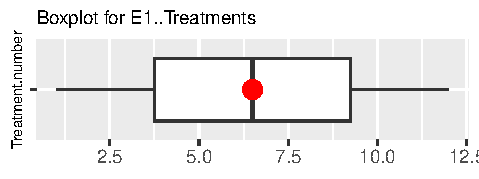
\includegraphics{FL_Crop_BMP_QA_single_dataset_files/figure-latex/check-content-of-sheets-1.pdf}
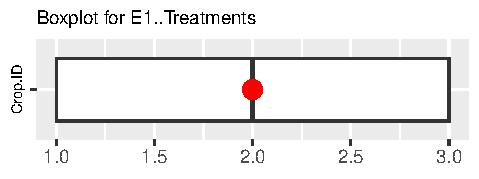
\includegraphics{FL_Crop_BMP_QA_single_dataset_files/figure-latex/check-content-of-sheets-2.pdf}
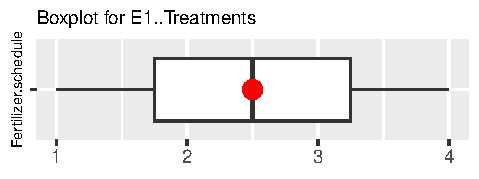
\includegraphics{FL_Crop_BMP_QA_single_dataset_files/figure-latex/check-content-of-sheets-3.pdf}
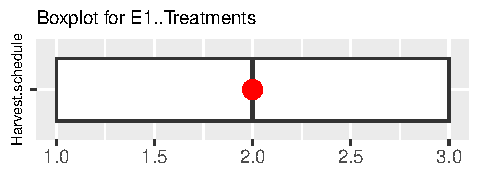
\includegraphics{FL_Crop_BMP_QA_single_dataset_files/figure-latex/check-content-of-sheets-4.pdf}

\begin{verbatim}


End of processing for E1..Treatments
*            ===================================================            *

START processing E2..Fields

 Variable           Value      Frequency
 Experiment ID      UFGA8201           1
 Site               UFGA               1
 Field location     1                  1
 Soil ID            IBPN910015         1
 Weather station ID UFGA               1
\end{verbatim}

\begin{verbatim}
End of processing for E2..Fields
*            ===================================================            *

START processing E3..Plots

 Variable      Value    Frequency
 Experiment ID UFGA8201        12
 Site          UFGA            12
\end{verbatim}

\begin{verbatim}
    Plot.ID      Treatment.number
 Min.   : 1.00   Min.   : 1.00   
 1st Qu.: 3.75   1st Qu.: 3.75   
 Median : 6.50   Median : 6.50   
 Mean   : 6.50   Mean   : 6.50   
 3rd Qu.: 9.25   3rd Qu.: 9.25   
 Max.   :12.00   Max.   :12.00   
\end{verbatim}

\begin{verbatim}
No id variables; using all as measure variables
\end{verbatim}

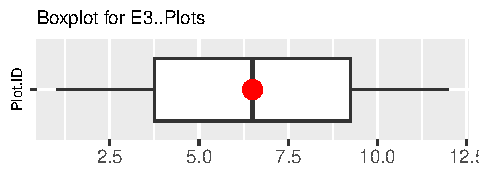
\includegraphics{FL_Crop_BMP_QA_single_dataset_files/figure-latex/check-content-of-sheets-5.pdf}
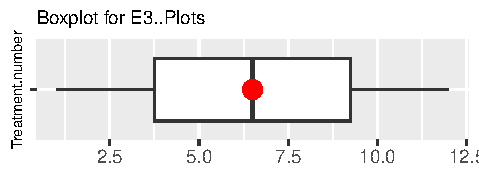
\includegraphics{FL_Crop_BMP_QA_single_dataset_files/figure-latex/check-content-of-sheets-6.pdf}

\begin{verbatim}


End of processing for E3..Plots
*            ===================================================            *

START processing E4..Crop.Information

 Variable            Value                     Frequency
 Experiment ID       UFGA8201                          3
 Site                UFGA                              3
 Crop species        Peanut                            3
 Cultivar            EARLY BUNCH                       1
 Cultivar            FLORUNNER, std                    1
 Cultivar            Non-Nodulated                     1
 Intended crop usage Cash crop                         1
 Intended crop usage Cover crop                        1
 Intended crop usage Seed                              1
 Cultivar notes      M4-2, non-nodulating line         1
\end{verbatim}

\begin{verbatim}
End of processing for E4..Crop.Information
*            ===================================================            *

START processing E5..Planting

 Variable              Value    Frequency
 Experiment ID         UFGA8201         1
 Site                  UFGA             1
 Planting material     dry seed         1
 Planting distribution row              1
\end{verbatim}

\begin{verbatim}
End of processing for E5..Planting
*            ===================================================            *

START processing E6..Irrigation

 Variable                    Value                                         Frequency
 Experiment ID               UFGA8201                                              1
 Site                        UFGA                                                  1
 Type of irrigation          sprinkle                                              1
 Notes related to irrigation Paper reports two irrigations, but original f         1
\end{verbatim}

\begin{verbatim}
End of processing for E6..Irrigation
*            ===================================================            *

START processing E7..Fertilizer

 Variable                    Value                                       Frequency
 Experiment ID               UFGA8201                                           17
 Site                        UFGA                                               17
 Nutrient Source             Ammonium nitrate                                    9
 Nutrient Source             compound fertilizer                                 4
 Nutrient Source             gypsum                                              4
 Placement                   broadcast                                           8
 Placement                   side-dressed                                        9
 Analysis                    ?                                                   4
 Analysis                    34:0:0                                              9
 Application timing          40 d                                                3
 Application timing          80 d                                                3
 Application timing          planting                                            3
 Application timing          pod initiation                                      4
 Application timing          preplant                                            4
 Notes related to applicatio 700 kg/ha. Date not given. Assuming 60 DAP.         4
 Notes related to applicatio Date not given                                      4
\end{verbatim}

\begin{verbatim}
 Fertilizer.schedule      Date            Amount.of.elemental.N.applied
 Min.   :1.000       Min.   :1982-05-10   Min.   : 0.00                
 1st Qu.:2.000       1st Qu.:1982-05-10   1st Qu.: 0.00                
 Median :2.000       Median :1982-06-19   Median :20.00                
 Mean   :2.471       Mean   :1982-06-15   Mean   :24.71                
 3rd Qu.:3.000       3rd Qu.:1982-07-15   3rd Qu.:40.00                
 Max.   :4.000       Max.   :1982-07-29   Max.   :80.00                
                                                                       
 Amount.of.elemental.P.applied Amount.of.elemental.K.applied Depth.of.incorporation
 Min.   :0.0000                Min.   :0.000                 Min.   : 0.000        
 1st Qu.:0.0000                1st Qu.:0.000                 1st Qu.: 0.000        
 Median :0.0000                Median :0.000                 Median : 0.000        
 Mean   :0.5882                Mean   :2.118                 Mean   : 4.615        
 3rd Qu.:0.0000                3rd Qu.:0.000                 3rd Qu.: 0.000        
 Max.   :2.5000                Max.   :9.000                 Max.   :20.000        
                                                             NA's   :4             
\end{verbatim}

\begin{verbatim}
No id variables; using all as measure variables
\end{verbatim}

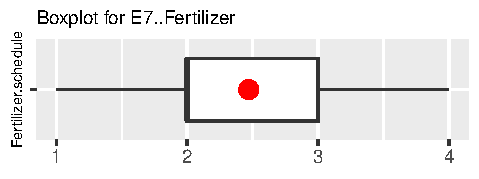
\includegraphics{FL_Crop_BMP_QA_single_dataset_files/figure-latex/check-content-of-sheets-7.pdf}
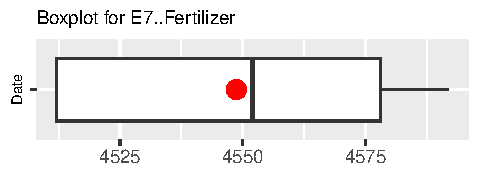
\includegraphics{FL_Crop_BMP_QA_single_dataset_files/figure-latex/check-content-of-sheets-8.pdf}
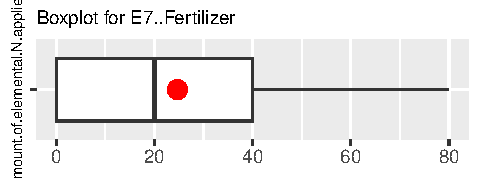
\includegraphics{FL_Crop_BMP_QA_single_dataset_files/figure-latex/check-content-of-sheets-9.pdf}
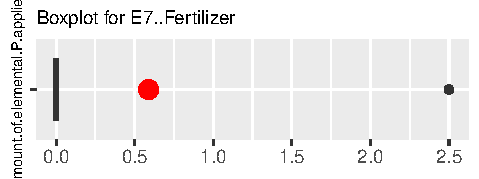
\includegraphics{FL_Crop_BMP_QA_single_dataset_files/figure-latex/check-content-of-sheets-10.pdf}
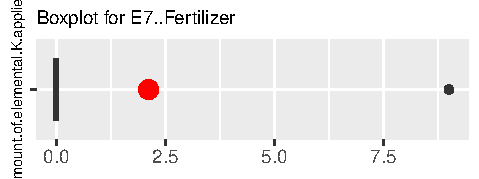
\includegraphics{FL_Crop_BMP_QA_single_dataset_files/figure-latex/check-content-of-sheets-11.pdf}
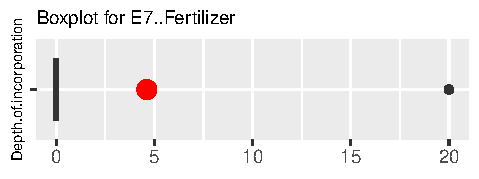
\includegraphics{FL_Crop_BMP_QA_single_dataset_files/figure-latex/check-content-of-sheets-12.pdf}

\begin{verbatim}


End of processing for E7..Fertilizer
*            ===================================================            *

START processing E9..Tillage

 Variable                   Value                                         Frequency
 Experiment ID              UFGA8201                                              3
 Site                       UFGA                                                  3
 Type of tillage operation  broadcast fertilizer application                      1
 Type of tillage operation  broadcast fertilizer application, gypsum              1
 Type of tillage operation  row planting with initial nitrogen                    1
 Notes related to operation "Preplant" but date not given. No information         1
 Notes related to operation 700 kg/ha. Date not given. Assuming 60 DAP.           1
 Notes related to operation Assuming one pass planting and side-dress             1
\end{verbatim}

\begin{verbatim}
End of processing for E9..Tillage
*            ===================================================            *

START processing E8..Organic.Amendments
\end{verbatim}

\begin{verbatim}
[1] Variable  Value     Frequency
<0 rows> (or 0-length row.names)

End of processing for E8..Organic.Amendments
*            ===================================================            *

START processing E10..Chemical.Applications

 Variable                    Value                                         Frequency
 Experiment ID               UFGA8201                                             10
 Site                        UFGA                                                 10
 Name of chemical applied    Balan (N-buthyl-N-ethyl-a-a-a-trifluro-2,6-di         1
 Name of chemical applied    Bravo (tetrachloroisothalonitrile)                    4
 Name of chemical applied    Sevin (1-naphyl N-methyl-carbamate)                   4
 Name of chemical applied    Vernam (S-propyl dipropylthio-carbamate)              1
 Chemicals application metho broadcast                                             2
 Chemicals application metho sprayed                                               8
 Notes related to applicatio  biweekly from 60 DAP to maturity                     8
 Notes related to applicatio "preplant", date is guess                             2
\end{verbatim}

\begin{verbatim}
      Date            Chemicals.application.amount
 Min.   :1982-05-05   Min.   :0.90                
 1st Qu.:1982-07-09   1st Qu.:1.36                
 Median :1982-07-23   Median :1.82                
 Mean   :1982-07-07   Mean   :1.82                
 3rd Qu.:1982-07-23   3rd Qu.:2.28                
 Max.   :1982-08-06   Max.   :2.74                
                      NA's   :8                   
\end{verbatim}

\begin{verbatim}
No id variables; using all as measure variables
\end{verbatim}

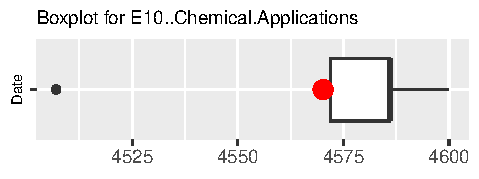
\includegraphics{FL_Crop_BMP_QA_single_dataset_files/figure-latex/check-content-of-sheets-13.pdf}
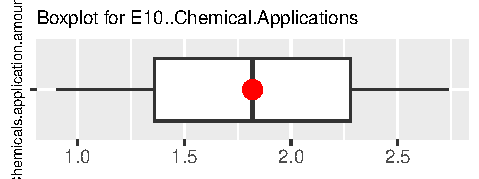
\includegraphics{FL_Crop_BMP_QA_single_dataset_files/figure-latex/check-content-of-sheets-14.pdf}

\begin{verbatim}


End of processing for E10..Chemical.Applications
*            ===================================================            *

START processing E11..Harvest

 Variable               Value    Frequency
 Experiment ID          UFGA8201         3
 Site                   UFGA             3
 Crop species harvested peanut           3
 Harvest component      seed             3
 Harvest method         hand             3
\end{verbatim}

\begin{verbatim}
End of processing for E11..Harvest
*            ===================================================            *

START processing E12..Preplant.Soil

 Variable      Value    Frequency
 Experiment ID UFGA8201         9
 Site          UFGA             9
\end{verbatim}

\begin{verbatim}
 Depth.of.measurement..top.of.soil.layer Depth.of.measurement..bottom.of.soil.layer
 Min.   :  0.00                          Min.   :  5.00                            
 1st Qu.: 15.00                          1st Qu.: 30.00                            
 Median : 45.00                          Median : 60.00                            
 Mean   : 57.22                          Mean   : 77.22                            
 3rd Qu.: 90.00                          3rd Qu.:120.00                            
 Max.   :150.00                          Max.   :180.00                            
 Soil.water.content   Ammonium.N   
 Min.   :0.0760     Min.   :0.500  
 1st Qu.:0.0860     1st Qu.:0.500  
 Median :0.0860     Median :1.500  
 Mean   :0.1078     Mean   :1.067  
 3rd Qu.:0.0860     3rd Qu.:1.500  
 Max.   :0.2580     Max.   :1.500  
\end{verbatim}

\begin{verbatim}
No id variables; using all as measure variables
\end{verbatim}

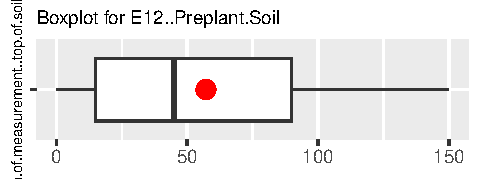
\includegraphics{FL_Crop_BMP_QA_single_dataset_files/figure-latex/check-content-of-sheets-15.pdf}
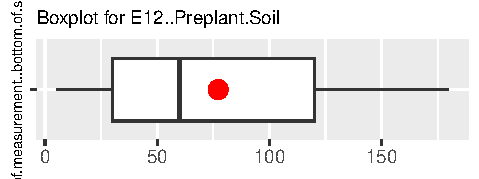
\includegraphics{FL_Crop_BMP_QA_single_dataset_files/figure-latex/check-content-of-sheets-16.pdf}
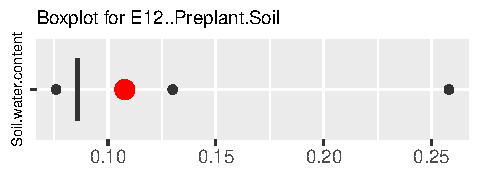
\includegraphics{FL_Crop_BMP_QA_single_dataset_files/figure-latex/check-content-of-sheets-17.pdf}
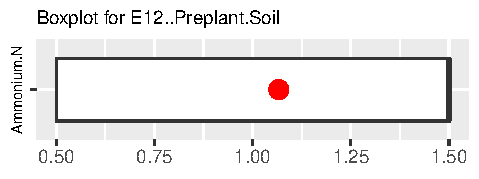
\includegraphics{FL_Crop_BMP_QA_single_dataset_files/figure-latex/check-content-of-sheets-18.pdf}

\begin{verbatim}


End of processing for E12..Preplant.Soil
*            ===================================================            *

START processing O1..Analysis.Methods
\end{verbatim}

\begin{verbatim}
[1] Variable  Value     Frequency
<0 rows> (or 0-length row.names)

End of processing for O1..Analysis.Methods
*            ===================================================            *

START processing O2..Yield.Summary

 Variable      Value    Frequency
 Experiment ID UFGA8201        12
 Site          UFGA            12
\end{verbatim}

\begin{verbatim}
    Plot.ID      Treatment.number   Seed.yield   Single.seed.wt    Seed.per.m2   
 Min.   : 1.00   Min.   : 1.00    Min.   : 680   Min.   :0.3560   Min.   :191.0  
 1st Qu.: 3.75   1st Qu.: 3.75    1st Qu.:1811   1st Qu.:0.4195   1st Qu.:238.8  
 Median : 6.50   Median : 6.50    Median :2108   Median :0.5820   Median :321.5  
 Mean   : 6.50   Mean   : 6.50    Mean   :1941   Mean   :0.6378   Mean   :317.8  
 3rd Qu.: 9.25   3rd Qu.: 9.25    3rd Qu.:2251   3rd Qu.:0.9187   3rd Qu.:383.2  
 Max.   :12.00   Max.   :12.00    Max.   :2714   Max.   :0.9470   Max.   :455.0  
                                                                                 
    LAI.max       Tops.dry.wt      Pod.dry.wt   Harvest.index    Pod.harvest.index
 Min.   :3.930   Min.   :10400   Min.   :1068   Min.   :0.0620   Min.   :0.0980   
 1st Qu.:4.207   1st Qu.:11600   1st Qu.:2570   1st Qu.:0.0865   1st Qu.:0.1227   
 Median :5.025   Median :16050   Median :2882   Median :0.1255   Median :0.1605   
 Mean   :5.220   Mean   :15350   Mean   :2664   Mean   :0.1331   Mean   :0.1837   
 3rd Qu.:6.037   3rd Qu.:18050   3rd Qu.:3024   3rd Qu.:0.1855   3rd Qu.:0.2597   
 Max.   :6.900   Max.   :21900   Max.   :3453   Max.   :0.2050   Max.   :0.2870   
 NA's   :8                                                                        
 Threshing.percent Tops.nitrogen   Seed.nitrogen.tot Seed.nitrogen.conc.
 Min.   :62.60     Min.   : 98.6   Min.   : 20.20    Min.   :2.970      
 1st Qu.:69.75     1st Qu.:190.9   1st Qu.: 65.62    1st Qu.:3.600      
 Median :71.65     Median :215.7   Median :105.70    Median :4.750      
 Mean   :72.18     Mean   :214.7   Mean   : 88.33    Mean   :4.353      
 3rd Qu.:76.83     3rd Qu.:259.3   3rd Qu.:110.50    3rd Qu.:4.935      
 Max.   :78.70     Max.   :301.3   Max.   :126.00    Max.   :5.240      
                                                                        
\end{verbatim}

\begin{verbatim}
No id variables; using all as measure variables
\end{verbatim}

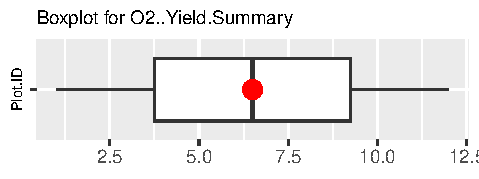
\includegraphics{FL_Crop_BMP_QA_single_dataset_files/figure-latex/check-content-of-sheets-19.pdf}
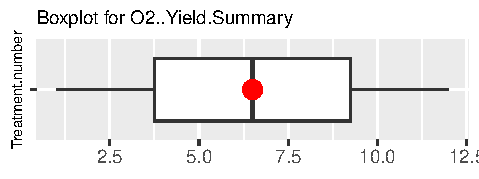
\includegraphics{FL_Crop_BMP_QA_single_dataset_files/figure-latex/check-content-of-sheets-20.pdf}
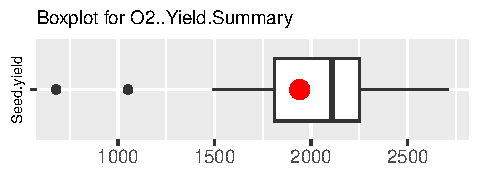
\includegraphics{FL_Crop_BMP_QA_single_dataset_files/figure-latex/check-content-of-sheets-21.pdf}
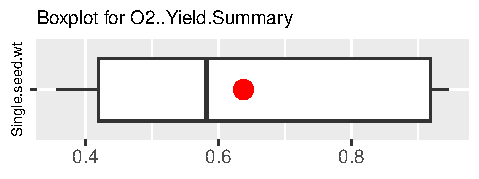
\includegraphics{FL_Crop_BMP_QA_single_dataset_files/figure-latex/check-content-of-sheets-22.pdf}
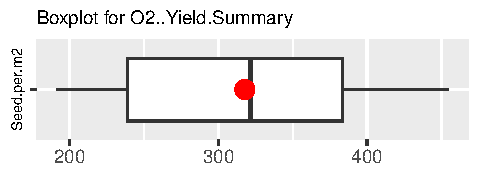
\includegraphics{FL_Crop_BMP_QA_single_dataset_files/figure-latex/check-content-of-sheets-23.pdf}
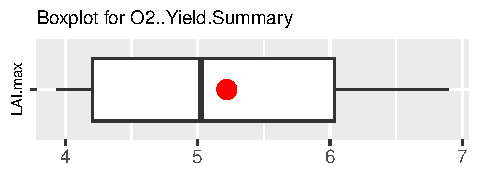
\includegraphics{FL_Crop_BMP_QA_single_dataset_files/figure-latex/check-content-of-sheets-24.pdf}
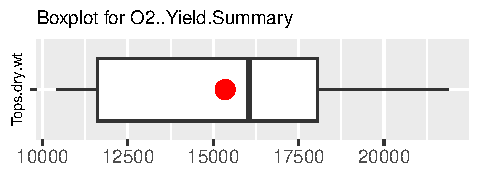
\includegraphics{FL_Crop_BMP_QA_single_dataset_files/figure-latex/check-content-of-sheets-25.pdf}
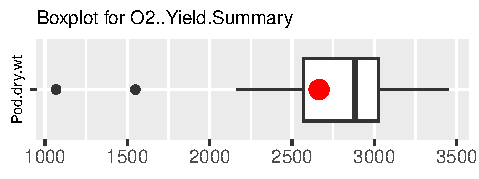
\includegraphics{FL_Crop_BMP_QA_single_dataset_files/figure-latex/check-content-of-sheets-26.pdf}
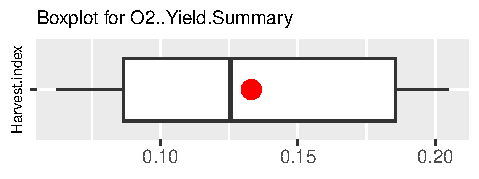
\includegraphics{FL_Crop_BMP_QA_single_dataset_files/figure-latex/check-content-of-sheets-27.pdf}
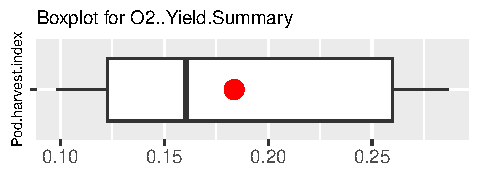
\includegraphics{FL_Crop_BMP_QA_single_dataset_files/figure-latex/check-content-of-sheets-28.pdf}
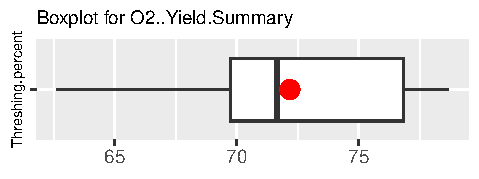
\includegraphics{FL_Crop_BMP_QA_single_dataset_files/figure-latex/check-content-of-sheets-29.pdf}
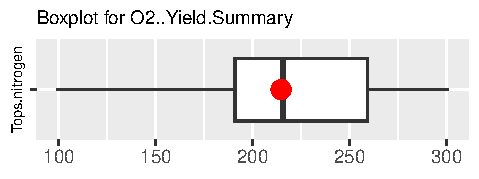
\includegraphics{FL_Crop_BMP_QA_single_dataset_files/figure-latex/check-content-of-sheets-30.pdf}
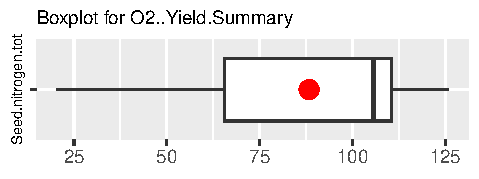
\includegraphics{FL_Crop_BMP_QA_single_dataset_files/figure-latex/check-content-of-sheets-31.pdf}
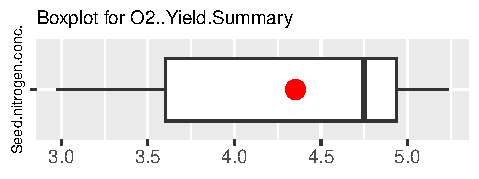
\includegraphics{FL_Crop_BMP_QA_single_dataset_files/figure-latex/check-content-of-sheets-32.pdf}

\begin{verbatim}


End of processing for O2..Yield.Summary
*            ===================================================            *

START processing O3..Crop.Growth

 Variable      Value    Frequency
 Experiment ID UFGA8201        28
 Site          UFGA            28
\end{verbatim}

\begin{verbatim}
 Treatment.number    Plot.ID       Sampling.date        Leaf.area.index  Tops.dry.weight
 Min.   : 1.000   Min.   : 1.000   Min.   :1982-06-29   Min.   :0.4200   Min.   :10400  
 1st Qu.: 2.000   1st Qu.: 2.000   1st Qu.:1982-07-09   1st Qu.:0.8025   1st Qu.:11600  
 Median : 3.000   Median : 3.000   Median :1982-08-13   Median :1.6900   Median :16050  
 Mean   : 4.214   Mean   : 4.214   Mean   :1982-08-18   Mean   :2.3065   Mean   :15350  
 3rd Qu.: 5.250   3rd Qu.: 5.250   3rd Qu.:1982-09-27   3rd Qu.:3.6725   3rd Qu.:18050  
 Max.   :12.000   Max.   :12.000   Max.   :1982-10-02   Max.   :6.9000   Max.   :21900  
                                                        NA's   :8        NA's   :16     
 Pod.dry.weight Seed.dry.weight Unit.seed.weight  Seed.number    Harvest.index   
 Min.   :1068   Min.   : 680    Min.   :356.0    Min.   :191.0   Min.   :0.0620  
 1st Qu.:2570   1st Qu.:1811    1st Qu.:419.5    1st Qu.:238.8   1st Qu.:0.0865  
 Median :2882   Median :2147    Median :582.0    Median :321.5   Median :0.1255  
 Mean   :2664   Mean   :1948    Mean   :637.8    Mean   :317.8   Mean   :0.1331  
 3rd Qu.:3024   3rd Qu.:2251    3rd Qu.:918.8    3rd Qu.:383.2   3rd Qu.:0.1855  
 Max.   :3453   Max.   :2714    Max.   :947.0    Max.   :455.0   Max.   :0.2050  
 NA's   :16     NA's   :16      NA's   :16       NA's   :16      NA's   :16      
 Pod.harvest.index Shelling.percent Tops.nitrogen   Leaf.nitrogen   Seed.nitrogen   
 Min.   :0.0980    Min.   :62.60    Min.   : 98.6   Min.   :32.40   Min.   : 20.20  
 1st Qu.:0.1227    1st Qu.:69.75    1st Qu.:190.9   1st Qu.:38.20   1st Qu.: 65.62  
 Median :0.1605    Median :71.65    Median :215.7   Median :47.30   Median :105.70  
 Mean   :0.1837    Mean   :72.18    Mean   :214.7   Mean   :50.38   Mean   : 88.33  
 3rd Qu.:0.2597    3rd Qu.:76.83    3rd Qu.:259.3   3rd Qu.:60.15   3rd Qu.:110.50  
 Max.   :0.2870    Max.   :78.70    Max.   :301.3   Max.   :75.90   Max.   :126.00  
 NA's   :16        NA's   :16       NA's   :16      NA's   :16      NA's   :16      
 Seed.N.concentration Leaf.N.concentration Stem.N.concentration
 Min.   :3.010        Min.   :1.930        Min.   :0.770       
 1st Qu.:3.600        1st Qu.:1.930        1st Qu.:0.770       
 Median :4.755        Median :2.910        Median :1.110       
 Mean   :4.341        Mean   :2.723        Mean   :1.047       
 3rd Qu.:4.942        3rd Qu.:3.330        3rd Qu.:1.260       
 Max.   :5.050        Max.   :3.330        Max.   :1.260       
 NA's   :16           NA's   :16           NA's   :16          
\end{verbatim}

\begin{verbatim}
No id variables; using all as measure variables
\end{verbatim}

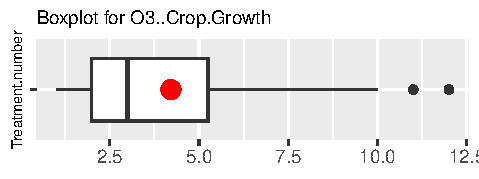
\includegraphics{FL_Crop_BMP_QA_single_dataset_files/figure-latex/check-content-of-sheets-33.pdf}
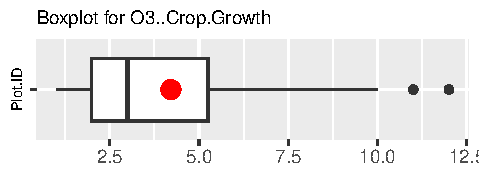
\includegraphics{FL_Crop_BMP_QA_single_dataset_files/figure-latex/check-content-of-sheets-34.pdf}
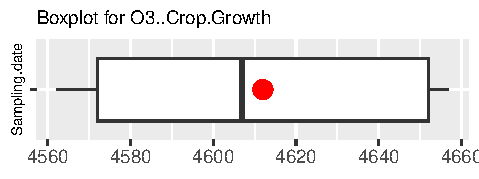
\includegraphics{FL_Crop_BMP_QA_single_dataset_files/figure-latex/check-content-of-sheets-35.pdf}
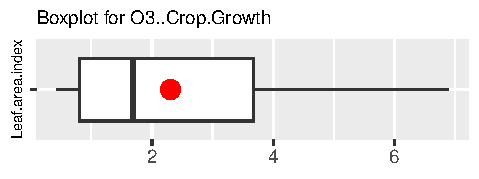
\includegraphics{FL_Crop_BMP_QA_single_dataset_files/figure-latex/check-content-of-sheets-36.pdf}
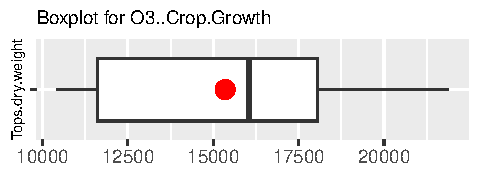
\includegraphics{FL_Crop_BMP_QA_single_dataset_files/figure-latex/check-content-of-sheets-37.pdf}
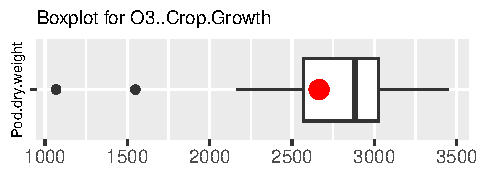
\includegraphics{FL_Crop_BMP_QA_single_dataset_files/figure-latex/check-content-of-sheets-38.pdf}
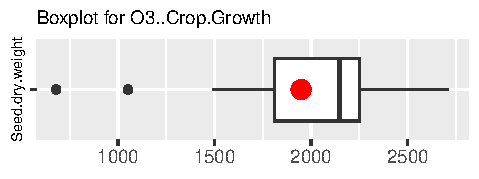
\includegraphics{FL_Crop_BMP_QA_single_dataset_files/figure-latex/check-content-of-sheets-39.pdf}
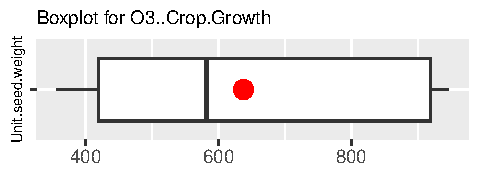
\includegraphics{FL_Crop_BMP_QA_single_dataset_files/figure-latex/check-content-of-sheets-40.pdf}
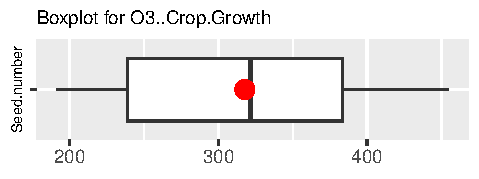
\includegraphics{FL_Crop_BMP_QA_single_dataset_files/figure-latex/check-content-of-sheets-41.pdf}
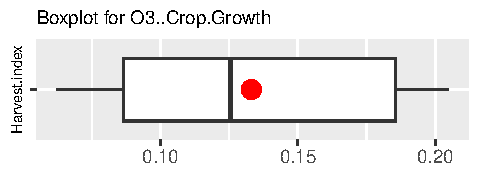
\includegraphics{FL_Crop_BMP_QA_single_dataset_files/figure-latex/check-content-of-sheets-42.pdf}
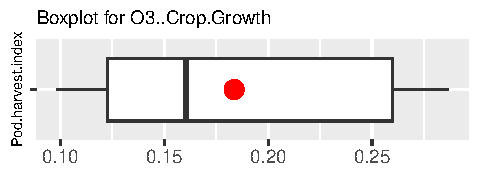
\includegraphics{FL_Crop_BMP_QA_single_dataset_files/figure-latex/check-content-of-sheets-43.pdf}
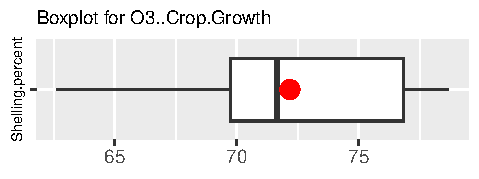
\includegraphics{FL_Crop_BMP_QA_single_dataset_files/figure-latex/check-content-of-sheets-44.pdf}
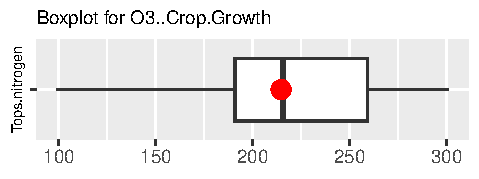
\includegraphics{FL_Crop_BMP_QA_single_dataset_files/figure-latex/check-content-of-sheets-45.pdf}
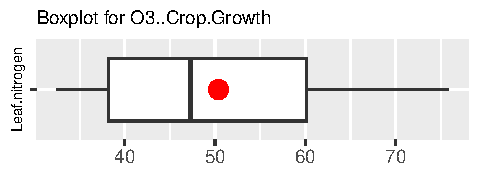
\includegraphics{FL_Crop_BMP_QA_single_dataset_files/figure-latex/check-content-of-sheets-46.pdf}
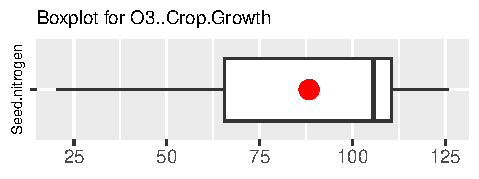
\includegraphics{FL_Crop_BMP_QA_single_dataset_files/figure-latex/check-content-of-sheets-47.pdf}
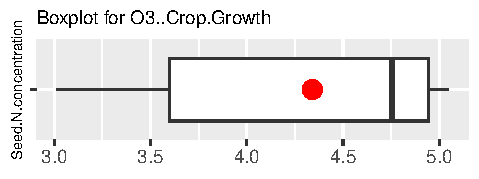
\includegraphics{FL_Crop_BMP_QA_single_dataset_files/figure-latex/check-content-of-sheets-48.pdf}
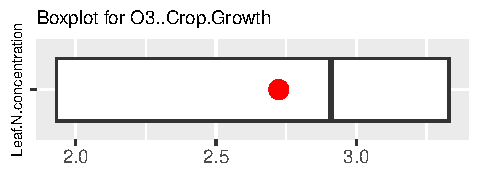
\includegraphics{FL_Crop_BMP_QA_single_dataset_files/figure-latex/check-content-of-sheets-49.pdf}
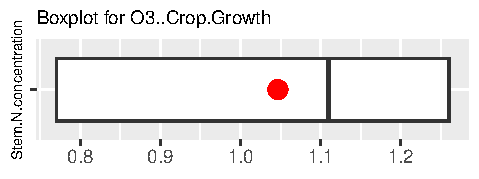
\includegraphics{FL_Crop_BMP_QA_single_dataset_files/figure-latex/check-content-of-sheets-50.pdf}

\begin{verbatim}


End of processing for O3..Crop.Growth
*            ===================================================            *

START processing O4..Crop.Health
\end{verbatim}

\begin{verbatim}
[1] Variable  Value     Frequency
<0 rows> (or 0-length row.names)

End of processing for O4..Crop.Health
*            ===================================================            *

START processing O5..Soil.Surface.Properties
\end{verbatim}

\begin{verbatim}
[1] Variable  Value     Frequency
<0 rows> (or 0-length row.names)

End of processing for O5..Soil.Surface.Properties
*            ===================================================            *

START processing O6..Soil.Layer.Properties
\end{verbatim}

\begin{verbatim}
[1] Variable  Value     Frequency
<0 rows> (or 0-length row.names)

End of processing for O6..Soil.Layer.Properties
*            ===================================================            *

START processing O7..Water
\end{verbatim}

\begin{verbatim}
[1] Variable  Value     Frequency
<0 rows> (or 0-length row.names)

End of processing for O7..Water
*            ===================================================            *

START processing S1..Soil.Metadata

 Variable                   Value                                 Frequency
 Soil ID                    IBPN910015                                    1
 Soil name                  Millhopper Fine Sand                          1
 Soil classification        Loamy,silic,hyperth Gross. Paleudults         1
 Soil classification system USDA                                          1
 Source of soil data        DSSAT                                         1
 Anonymize                  N                                             1
\end{verbatim}

\begin{verbatim}
End of processing for S1..Soil.Metadata
*            ===================================================            *

START processing S2..Soil.Layer.Properties

 Variable Value      Frequency
  Soil ID IBPN910015         9
\end{verbatim}

\begin{verbatim}
 Top.of.soil.layer Bottom.of.soil.layer      Clay            Silt             Sand      
 Min.   :  0.00    Min.   :  5.00       Min.   :0.900   Min.   : 3.600   Min.   :86.20  
 1st Qu.: 15.00    1st Qu.: 30.00       1st Qu.:4.600   1st Qu.: 4.200   1st Qu.:87.30  
 Median : 45.00    Median : 60.00       Median :5.800   Median : 5.400   Median :88.10  
 Mean   : 57.22    Mean   : 77.22       Mean   :5.978   Mean   : 6.267   Mean   :87.76  
 3rd Qu.: 90.00    3rd Qu.:120.00       3rd Qu.:8.300   3rd Qu.: 6.400   3rd Qu.:88.80  
 Max.   :150.00    Max.   :180.00       Max.   :9.600   Max.   :11.800   Max.   :89.00  
 Organic.matter    Bulk.density   Wilting.point     Field.capacity  
 Min.   :0.0300   Min.   :1.360   Min.   :0.02000   Min.   :0.0760  
 1st Qu.:0.0300   1st Qu.:1.430   1st Qu.:0.02300   1st Qu.:0.0860  
 Median :0.2000   Median :1.460   Median :0.02300   Median :0.0860  
 Mean   :0.2722   Mean   :1.491   Mean   :0.02811   Mean   :0.1078  
 3rd Qu.:0.2800   3rd Qu.:1.480   3rd Qu.:0.02300   3rd Qu.:0.0860  
 Max.   :0.9000   Max.   :1.790   Max.   :0.07000   Max.   :0.2580  
 Saturated.hydraulic.conductivity
 Min.   : 0.10                   
 1st Qu.: 7.40                   
 Median :15.80                   
 Mean   :14.68                   
 3rd Qu.:27.60                   
 Max.   :28.00                   
\end{verbatim}

\begin{verbatim}
No id variables; using all as measure variables
\end{verbatim}

\includegraphics{FL_Crop_BMP_QA_single_dataset_files/figure-latex/check-content-of-sheets-51.pdf}
\includegraphics{FL_Crop_BMP_QA_single_dataset_files/figure-latex/check-content-of-sheets-52.pdf}
\includegraphics{FL_Crop_BMP_QA_single_dataset_files/figure-latex/check-content-of-sheets-53.pdf}
\includegraphics{FL_Crop_BMP_QA_single_dataset_files/figure-latex/check-content-of-sheets-54.pdf}
\includegraphics{FL_Crop_BMP_QA_single_dataset_files/figure-latex/check-content-of-sheets-55.pdf}
\includegraphics{FL_Crop_BMP_QA_single_dataset_files/figure-latex/check-content-of-sheets-56.pdf}
\includegraphics{FL_Crop_BMP_QA_single_dataset_files/figure-latex/check-content-of-sheets-57.pdf}
\includegraphics{FL_Crop_BMP_QA_single_dataset_files/figure-latex/check-content-of-sheets-58.pdf}
\includegraphics{FL_Crop_BMP_QA_single_dataset_files/figure-latex/check-content-of-sheets-59.pdf}
\includegraphics{FL_Crop_BMP_QA_single_dataset_files/figure-latex/check-content-of-sheets-60.pdf}

\begin{verbatim}


End of processing for S2..Soil.Layer.Properties
*            ===================================================            *

START processing W1..Weather.Station.Metadata

 Variable             Value                   Frequency
 Weather station ID   UFGA                            1
 Weather station name Gainesville,Florida,USA         1
 Anonymize            N                               1
\end{verbatim}

\begin{verbatim}
End of processing for W1..Weather.Station.Metadata
*            ===================================================            *

START processing W2..Daily.Weather.Data

 Variable           Value Frequency
 Weather station ID  UFGA       365
\end{verbatim}

\begin{verbatim}
      Date            Minimum.daily.air.temperature Maximum.daily.air.temperature
 Min.   :1982-01-01   Min.   :-7.80                 Min.   :10.00                
 1st Qu.:1982-04-02   1st Qu.:12.80                 1st Qu.:25.60                
 Median :1982-07-02   Median :16.70                 Median :28.90                
 Mean   :1982-07-02   Mean   :15.69                 Mean   :28.27                
 3rd Qu.:1982-10-01   3rd Qu.:21.10                 3rd Qu.:32.20                
 Max.   :1982-12-31   Max.   :26.10                 Max.   :35.60                
 Daily.precipitation Solar.radiation      PAR       
 Min.   : 0.000      Min.   : 0.80   Min.   : 2.20  
 1st Qu.: 0.000      1st Qu.:10.30   1st Qu.:22.00  
 Median : 0.000      Median :14.00   Median :28.00  
 Mean   : 4.232      Mean   :14.65   Mean   :29.66  
 3rd Qu.: 1.300      3rd Qu.:19.00   3rd Qu.:37.60  
 Max.   :98.800      Max.   :26.90   Max.   :57.20  
\end{verbatim}

\begin{verbatim}
No id variables; using all as measure variables
\end{verbatim}

\includegraphics{FL_Crop_BMP_QA_single_dataset_files/figure-latex/check-content-of-sheets-61.pdf}
\includegraphics{FL_Crop_BMP_QA_single_dataset_files/figure-latex/check-content-of-sheets-62.pdf}
\includegraphics{FL_Crop_BMP_QA_single_dataset_files/figure-latex/check-content-of-sheets-63.pdf}
\includegraphics{FL_Crop_BMP_QA_single_dataset_files/figure-latex/check-content-of-sheets-64.pdf}
\includegraphics{FL_Crop_BMP_QA_single_dataset_files/figure-latex/check-content-of-sheets-65.pdf}
\includegraphics{FL_Crop_BMP_QA_single_dataset_files/figure-latex/check-content-of-sheets-66.pdf}

\begin{verbatim}


End of processing for W2..Daily.Weather.Data
*            ===================================================            *
\end{verbatim}

\begin{center}\rule{0.5\linewidth}{0.5pt}\end{center}

\subsection{2.2. Correct Dates? Are events sequenced as
expected?}\label{correct-dates-are-events-sequenced-as-expected}

Dates of key management events such as plantings, irrigations and
harvests are sometimes entered incorrectly. A common problem is
inversion of days and months (is `3/5' ``March 5'' or ``3 April''?). To
check dates, we plot management events for each combination of
Experiment, Site and Year along a timeline. To reduce the potential
number of plots, data from different treatments and replicates are
pooled together. This means some timelines may include multiple
instances of plantings, fertilizer applications, harvests or other
events. We currently do not consider crop phenology such as flowering or
maturity dates.

\begin{verbatim}
Warning: Removed 1 row containing missing values or values outside the scale range
(`geom_point()`).
\end{verbatim}

\begin{verbatim}
Warning: Removed 1 row containing missing values or values outside the scale range
(`geom_text()`).
\end{verbatim}

\includegraphics{FL_Crop_BMP_QA_single_dataset_files/figure-latex/check-dates-1.pdf}

\newpage

\subsection{2.3. Correct geocoordinates? Are locations mapped as
expected?}\label{correct-geocoordinates-are-locations-mapped-as-expected}

Experience shows that datasets often have errors in location data. This
section checks that any reported geocoordinates are roughly correct by
mapping. Geocoordinates may appear in four sheets:

\begin{itemize}
\tightlist
\item
  M2. Sites
\item
  E2. Fields
\item
  S1. Soil Metadata
\item
  W1. Weather Station Metadata
\end{itemize}

To facilitate processing, we extract the geocoordinates and the location
name, and add as `Source' the name of the individual sheet containing
the data.

\begin{center}\rule{0.5\linewidth}{0.5pt}\end{center}

\subsubsection{2.3.1. List of all expected
geocoordinates}\label{list-of-all-expected-geocoordinates}

\begin{verbatim}
 Source        Location   Lat       Long      
 M2. Sites     UFGA        29.63696  -82.37041
 E2. Fields    1                 NA         NA
 S1. Soil Meta IBPN910015  29.63000  -82.37000
 W1. Weather   UFGA        29.63000  -82.37000
\end{verbatim}

\begin{center}\rule{0.5\linewidth}{0.5pt}\end{center}

\subsubsection{2.3.2. Displaying the reference map of Florida with any
reported
locations}\label{displaying-the-reference-map-of-florida-with-any-reported-locations}

Here we use a map of Florida as the base. If latitude or longitude
values are very far off (e.g., if the values are reversed or longitude
is assigned a positive value for anywhere in the Americas), the map will
display, but it may be distorted and not look like the expected base map
of Florida.

\begin{verbatim}
Warning: Removed 1 row containing missing values or values outside the scale range
(`geom_point()`).
\end{verbatim}

\includegraphics{FL_Crop_BMP_QA_single_dataset_files/figure-latex/map-geocoords-1.pdf}

The option position = position\_jitter is used so that if there are a
large number of points with nearly identical locations, these are spread
out slightly.

\newpage

\subsection{2.4. Completeness of sheets: Checking whether sheets present
in the template are missing from the
dataset}\label{completeness-of-sheets-checking-whether-sheets-present-in-the-template-are-missing-from-the-dataset}

Users may add sheets as needed but are discouraged from deleting sheets.

\begin{verbatim}
The sheet names match.
\end{verbatim}

\subsection{2.5. Completeness of data in individual
sheets}\label{completeness-of-data-in-individual-sheets}

To assess completeness, we need to know whether most of the variables
actually have data values (e.g., are not empty cells). Below is a count
of total values for variables used in each sheet. To avoid the output
being split into two sections, variable names that are longer than 30
characters are truncated.

\begin{verbatim}
Total Non-Missing Values across all sheets: 4286 
\end{verbatim}

\begin{verbatim}
Total Missing Values across all sheets: 811 
\end{verbatim}

\begin{verbatim}
 Sheet_name                   Variable                       Non_NA Missing
 M1. Experiments              Experiment name                     1       0
 M1. Experiments              Experiment ID                       1       0
 M1. Experiments              Research data owner                 1       0
 M1. Experiments              Institutional data owner            1       0
 M1. Experiments              Contributor e-mail                  0       1
 M1. Experiments              Publication journal & volume        1       0
 M1. Experiments              Link to document                    1       0
 M1. Experiments              Publication DOI                     1       0
 M1. Experiments              Should data be anonymized?          1       0
 M1. Experiments              Data release date                   0       1
 M2. Sites                    Site                                1       0
 M2. Sites                    Local name for experiment site      1       0
 M2. Sites                    State                               1       0
 M2. Sites                    County                              1       0
 M2. Sites                    Town or other                       1       0
 M2. Sites                    Latitude                            1       0
 M2. Sites                    Longitude                           1       0
 M3. Experimental Design      Experiment ID                       1       0
 M3. Experimental Design      Site                                1       0
 M3. Experimental Design      Rate treatments                     1       0
 M3. Experimental Design      Replicates                          1       0
 M3. Experimental Design      Treatment structure                 1       0
 M3. Experimental Design      Type of experiment                  1       0
 M3. Experimental Design      Main effect 1                       1       0
 M3. Experimental Design      Main effect 2                       1       0
 M3. Experimental Design      Plot width                          0       1
 M3. Experimental Design      Plot length                         1       0
 E1. Treatments               Treatment number                   12       0
 E1. Treatments               Treatment name                     12       0
 E1. Treatments               Experiment ID                      12       0
 E1. Treatments               Site                               12       0
 E1. Treatments               Field location                     12       0
 E1. Treatments               Study year                         12       0
 E1. Treatments               Crop ID                            12       0
 E1. Treatments               Planting schedule                  12       0
 E1. Treatments               Irrigation schedule                12       0
 E1. Treatments               Fertilizer schedule                12       0
 E1. Treatments               Organic amendments schedule        12       0
 E1. Treatments               Chemical applications schedule     12       0
 E1. Treatments               Tillage schedule                   12       0
 E1. Treatments               Harvest schedule                   12       0
 E1. Treatments               Soil initial conditions ID         12       0
 E1. Treatments               Comments about treatment            0      12
 E2. Fields                   Experiment ID                       1       0
 E2. Fields                   Site                                1       0
 E2. Fields                   Field location                      1       0
 E2. Fields                   Latitude                            0       1
 E2. Fields                   Longitude                           0       1
 E2. Fields                   Soil ID                             1       0
 E2. Fields                   Weather station ID                  1       0
 E2. Fields                   Distance to weather station         0       1
 E2. Fields                   Field area                          0       1
 E2. Fields                   Field length to width ratio         0       1
 E2. Fields                   Field slope                         0       1
 E2. Fields                   Drainage type                       0       1
 E2. Fields                   Water table depth                   0       1
 E2. Fields                   Type of organic matter              0       1
 E2. Fields                   Dry mass of surface organic ma      1       0
 E2. Fields                   Nitrogen concentration in surf      1       0
 E2. Fields                   Phosphorus concentration in su      1       0
 E2. Fields                   Portion of residue incorporate      1       0
 E2. Fields                   Depth of residue incorporation      1       0
 E3. Plots                    Plot ID                            12       0
 E3. Plots                    Experiment ID                      12       0
 E3. Plots                    Site                               12       0
 E3. Plots                    Field location                     12       0
 E3. Plots                    Treatment number                   12       0
 E3. Plots                    Replicate                          12       0
 E4. Crop Information         Experiment ID                       3       0
 E4. Crop Information         Site                                3       0
 E4. Crop Information         Year                                3       0
 E4. Crop Information         Crop ID                             3       0
 E4. Crop Information         Crop species                        3       0
 E4. Crop Information         Cultivar                            3       0
 E4. Crop Information         Intended crop usage                 3       0
 E4. Crop Information         Cultivar notes                      1       2
 E5. Planting                 Experiment ID                       1       0
 E5. Planting                 Site                                1       0
 E5. Planting                 Year                                1       0
 E5. Planting                 Planting schedule                   1       0
 E5. Planting                 Planting date                       1       0
 E5. Planting                 Row spacing                         1       0
 E5. Planting                 Planting density                    1       0
 E5. Planting                 Plant density at emergence          0       1
 E5. Planting                 Planting material                   1       0
 E5. Planting                 Planting distribution               1       0
 E6. Irrigation               Experiment ID                       1       0
 E6. Irrigation               Site                                1       0
 E6. Irrigation               Year                                1       0
 E6. Irrigation               Irrigation schedule                 1       0
 E6. Irrigation               Date of irrigation                  1       0
 E6. Irrigation               Type of irrigation                  1       0
 E6. Irrigation               Amount of irrigation                1       0
 E6. Irrigation               Notes related to irrigation         1       0
 E7. Fertilizer               Experiment ID                      17       0
 E7. Fertilizer               Site                               17       0
 E7. Fertilizer               Year                               17       0
 E7. Fertilizer               Fertilizer schedule                17       0
 E7. Fertilizer               Date                               17       0
 E7. Fertilizer               Nutrient Source                    17       0
 E7. Fertilizer               Amount of elemental N applied      17       0
 E7. Fertilizer               Amount of elemental P applied      17       0
 E7. Fertilizer               Amount of elemental K applied      17       0
 E7. Fertilizer               Placement                          17       0
 E7. Fertilizer               Depth of incorporation             13       4
 E7. Fertilizer               Analysis                           13       4
 E7. Fertilizer               Application timing                 17       0
 E7. Fertilizer               Notes related to application        8       9
 E9. Tillage                  Experiment ID                       3       0
 E9. Tillage                  Site                                3       0
 E9. Tillage                  Year                                3       0
 E9. Tillage                  Tillage schedule                    3       0
 E9. Tillage                  Date                                3       0
 E9. Tillage                  Type of tillage operation           3       0
 E9. Tillage                  Depth of incorporation              3       0
 E9. Tillage                  Notes related to operation          3       0
 E8. Organic Amendments       Experiment ID                       0       0
 E8. Organic Amendments       Site                                0       0
 E8. Organic Amendments       Year                                0       0
 E8. Organic Amendments       Organic amendments schedule         0       0
 E8. Organic Amendments       Date                                0       0
 E8. Organic Amendments       Type of organic matter              0       0
 E8. Organic Amendments       Amount of organic matter            0       0
 E8. Organic Amendments       Placement                           0       0
 E8. Organic Amendments       Depth of incorporation              0       0
 E8. Organic Amendments       N concentration                     0       0
 E8. Organic Amendments       Notes related to application        0       0
 E10. Chemical Applications   Experiment ID                      10       0
 E10. Chemical Applications   Site                               10       0
 E10. Chemical Applications   Year                               10       0
 E10. Chemical Applications   Chemical application schedule      10       0
 E10. Chemical Applications   Date                               10       0
 E10. Chemical Applications   Name of chemical applied           10       0
 E10. Chemical Applications   Chemicals application amount       10       0
 E10. Chemical Applications   Chemicals application method       10       0
 E10. Chemical Applications   Depth of application               10       0
 E10. Chemical Applications   Chemicals application target        0      10
 E10. Chemical Applications   Notes related to application       10       0
 E11. Harvest                 Experiment ID                       3       0
 E11. Harvest                 Site                                3       0
 E11. Harvest                 Year                                3       0
 E11. Harvest                 Harvest schedule                    3       0
 E11. Harvest                 Harvest date                        0       3
 E11. Harvest                 Crop species harvested              3       0
 E11. Harvest                 Harvest component                   3       0
 E11. Harvest                 Harvest method                      3       0
 E11. Harvest                 Main product harvested              3       0
 E11. Harvest                 By-product harvested                3       0
 E12. Preplant Soil           Experiment ID                       9       0
 E12. Preplant Soil           Site                                9       0
 E12. Preplant Soil           Year                                9       0
 E12. Preplant Soil           Soil initial conditions ID          9       0
 E12. Preplant Soil           Sampling date                       9       0
 E12. Preplant Soil           Depth of measurement, top of s      9       0
 E12. Preplant Soil           Depth of measurement, bottom o      9       0
 E12. Preplant Soil           Soil water content                  9       0
 E12. Preplant Soil           Nitrate N                           9       0
 E12. Preplant Soil           Ammonium N                          9       0
 E12. Preplant Soil           Stable organic C                    0       9
 O1. Analysis Methods         Experiment ID                       0       0
 O1. Analysis Methods         Full parameter name                 0       0
 O1. Analysis Methods         Header name (in data file)          0       0
 O1. Analysis Methods         Unit                                0       0
 O1. Analysis Methods         Matrix                              0       0
 O1. Analysis Methods         Analytical laboratory               0       0
 O1. Analysis Methods         Analysis method                     0       0
 O1. Analysis Methods         EPA method                          0       0
 O1. Analysis Methods         Computation method                  0       0
 O2. Yield Summary            Experiment ID                      12       0
 O2. Yield Summary            Site                               12       0
 O2. Yield Summary            Year                               12       0
 O2. Yield Summary            Plot ID                            12       0
 O2. Yield Summary            Treatment number                   12       0
 O2. Yield Summary            Replicate                           0      12
 O2. Yield Summary            Seed yield                         12       0
 O2. Yield Summary            Single seed wt                     12       0
 O2. Yield Summary            Seed per m2                        12       0
 O2. Yield Summary            LAI max                            12       0
 O2. Yield Summary            Tops dry wt                        12       0
 O2. Yield Summary            Pod dry wt                         12       0
 O2. Yield Summary            Harvest index                      12       0
 O2. Yield Summary            Pod harvest index                  12       0
 O2. Yield Summary            Threshing percent                  12       0
 O2. Yield Summary            Tops nitrogen                      12       0
 O2. Yield Summary            Seed nitrogen tot                  12       0
 O2. Yield Summary            Seed nitrogen conc.                12       0
 O3. Crop Growth              Experiment ID                      28       0
 O3. Crop Growth              Site                               28       0
 O3. Crop Growth              Year                               28       0
 O3. Crop Growth              Treatment number                   28       0
 O3. Crop Growth              Replicate                          28       0
 O3. Crop Growth              Plot ID                            28       0
 O3. Crop Growth              Sampling date                      28       0
 O3. Crop Growth              Leaf area index                    28       0
 O3. Crop Growth              Tops dry weight                    28       0
 O3. Crop Growth              Pod dry weight                     28       0
 O3. Crop Growth              Seed dry weight                    28       0
 O3. Crop Growth              Unit seed weight                   28       0
 O3. Crop Growth              Seed number                        28       0
 O3. Crop Growth              Harvest index                      28       0
 O3. Crop Growth              Pod harvest index                  28       0
 O3. Crop Growth              Shelling percent                   28       0
 O3. Crop Growth              Tops nitrogen                      28       0
 O3. Crop Growth              Leaf nitrogen                      28       0
 O3. Crop Growth              Seed nitrogen                      28       0
 O3. Crop Growth              Seed N concentration               28       0
 O3. Crop Growth              Leaf N concentration               28       0
 O3. Crop Growth              Stem N concentration               28       0
 O4. Crop Health              Experiment ID                       0       0
 O4. Crop Health              Site                                0       0
 O4. Crop Health              Year                                0       0
 O4. Crop Health              Treatment number                    0       0
 O4. Crop Health              Replicate                           0       0
 O4. Crop Health              Plot ID                             0       0
 O4. Crop Health              Sampling date                       0       0
 O4. Crop Health              Field notes                         0       0
 O5. Soil Surface Properties  Experiment ID                       0       0
 O5. Soil Surface Properties  Site                                0       0
 O5. Soil Surface Properties  Year                                0       0
 O5. Soil Surface Properties  Treatment number                    0       0
 O5. Soil Surface Properties  Replicate                           0       0
 O5. Soil Surface Properties  Plot ID                             0       0
 O5. Soil Surface Properties  Sampling date                       0       0
 O5. Soil Surface Properties  Type of organic matter              0       0
 O5. Soil Surface Properties  Dry mass of surface organic ma      0       0
 O5. Soil Surface Properties  Nitrogen concentration in surf      0       0
 O5. Soil Surface Properties  Phosphorus concentration in su      0       0
 O5. Soil Surface Properties  Potassium concentration in sur      0       0
 O6. Soil Layer Properties    Experiment ID                       0       0
 O6. Soil Layer Properties    Site                                0       0
 O6. Soil Layer Properties    Year                                0       0
 O6. Soil Layer Properties    Treatment number                    0       0
 O6. Soil Layer Properties    Replicate                           0       0
 O6. Soil Layer Properties    Plot ID                             0       0
 O6. Soil Layer Properties    Sampling date                       0       0
 O6. Soil Layer Properties    Depth of measurement, top of s      0       0
 O6. Soil Layer Properties    Depth of measurement, bottom o      0       0
 O6. Soil Layer Properties    Soil water content                  0       0
 O6. Soil Layer Properties    Nitrate N                           0       0
 O6. Soil Layer Properties    Ammonium N                          0       0
 O6. Soil Layer Properties    Total mineral N                     0       0
 O6. Soil Layer Properties    pH                                  0       0
 O6. Soil Layer Properties    Cation exchange capacity            0       0
 O6. Soil Layer Properties    Extractable P                       0       0
 O6. Soil Layer Properties    Potassium                           0       0
 O6. Soil Layer Properties    Magnesium                           0       0
 O6. Soil Layer Properties    Exchangeable Ca                     0       0
 O6. Soil Layer Properties    Potassium base saturation           0       0
 O6. Soil Layer Properties    Magnesium base saturation           0       0
 O6. Soil Layer Properties    Calcium base saturation             0       0
 O6. Soil Layer Properties    Hydrogen base saturation            0       0
 O7. Water                    Experiment ID                       0       0
 O7. Water                    Site                                0       0
 O7. Water                    Year                                0       0
 O7. Water                    Treatment number                    0       0
 O7. Water                    Replicate                           0       0
 O7. Water                    Plot ID                             0       0
 O7. Water                    Sampling date                       0       0
 O7. Water                    Sampling depth                      0       0
 O7. Water                    Row position                        0       0
 O7. Water                    Sampling method                     0       0
 O7. Water                    NO3-N conc                          0       0
 O7. Water                    Ammonium-N conc                     0       0
 O7. Water                    Total Kjeldahl N conc               0       0
 O7. Water                    Water sample notes                  0       0
 S1. Soil Metadata            Soil ID                             1       0
 S1. Soil Metadata            Soil name                           1       0
 S1. Soil Metadata            Soil classification                 1       0
 S1. Soil Metadata            Soil classification system          1       0
 S1. Soil Metadata            Source of soil data                 1       0
 S1. Soil Metadata            Latitude                            1       0
 S1. Soil Metadata            Longitude                           1       0
 S1. Soil Metadata            Elevation                           1       0
 S1. Soil Metadata            Anonymize                           1       0
 S1. Soil Metadata            Slope                               0       1
 S1. Soil Metadata            Soil surface color                  0       1
 S2. Soil Layer Properties    Soil ID                             9       0
 S2. Soil Layer Properties    Top of soil layer                   9       0
 S2. Soil Layer Properties    Bottom of soil layer                9       0
 S2. Soil Layer Properties    Clay                                9       0
 S2. Soil Layer Properties    Silt                                9       0
 S2. Soil Layer Properties    Sand                                9       0
 S2. Soil Layer Properties    Gravel                              9       0
 S2. Soil Layer Properties    Organic matter                      9       0
 S2. Soil Layer Properties    Bulk density                        9       0
 S2. Soil Layer Properties    Wilting point                       9       0
 S2. Soil Layer Properties    Field capacity                      9       0
 S2. Soil Layer Properties    Saturated hydraulic conductivi      9       0
 W1. Weather Station Metadata Weather station ID                  1       0
 W1. Weather Station Metadata Weather station name                1       0
 W1. Weather Station Metadata Latitude of station                 1       0
 W1. Weather Station Metadata Longitude of station                1       0
 W1. Weather Station Metadata Elevation of weather station        1       0
 W1. Weather Station Metadata Anonymize                           1       0
 W1. Weather Station Metadata Weather station temperature se      1       0
 W1. Weather Station Metadata Weather station link                0       1
 W2. Daily Weather Data       Weather station ID                365       0
 W2. Daily Weather Data       Date                              365       0
 W2. Daily Weather Data       Minimum daily air temperature     365       0
 W2. Daily Weather Data       Maximum daily air temperature     365       0
 W2. Daily Weather Data       Daily precipitation               365       0
 W2. Daily Weather Data       Solar radiation                   365       0
 W2. Daily Weather Data       Temperature, dewpoint               0     365
 W2. Daily Weather Data       Wind speed, daily                   0     365
 W2. Daily Weather Data       PAR                               365       0
\end{verbatim}

\newpage

\section{3.0. Coherent Identifiers?}\label{coherent-identifiers}

Index variables (`keys' in database terminology) from pairs of data
frames are compared to make sure that the index values are identical
across the sheets. This is fundamental to allowing different types of
data to be linked across sheets. For example the values of `Field
location' should be the same in the sheets `E1. Treatments' and `E2.
Fields'.

The basic approach for testing:

\begin{enumerate}
\def\labelenumi{\arabic{enumi}.}
\tightlist
\item
  Create two temporary data frames.
\item
  Merge the data frames based on identifiers given as a list in the
  argument `TestVar'.
\item
  Reduce the two data frames to just the columns corresponding to
  `TestVar'.
\item
  Extract the unique combinations of values for each data frame.
\item
  Add flag variables, `from\_df1' and `from\_df2', to make it easier to
  detect problems.
\item
  Merge the the two data frames to create `dfMerged'.
\item
  Compare the length of the two data frames. The lengths should be
  identical.
\item
  Print the merged test dataset `dfMerged' to allow inspection by the
  users.
\end{enumerate}

If the two frames are of different lengths, then there is a problem. If
the two data frames are of the same length, one should still review
`from\_df1' and `from\_df2' to see whether there are mismatches, which
would be indicated by `NA' in one of the two columns.

Common sources of mismatches include:

\begin{itemize}
\tightlist
\item
  Inconsistent use of spaces such as `Blk 1' vs.~`Blk1'.
\item
  Simple spelling errors (`Fred' vs.~`Frred')
\item
  Experiments, treatments or plots that were either never planted or not
  harvested.
\item
  Extra rows being read in a given sheet, leading to an empty cell being
  assigned a value of NA. This may arise if a stray character appears
  outside of the intended range of data.
\end{itemize}

In the third case, it is helpful to provide a comment or note in the
appropriate sheets.

\newpage

\subsection{3.1. Comparing identifiers used in M1. Experiments, E1.
Treatments, E2. Fields and E3.
Plots}\label{comparing-identifiers-used-in-m1.-experiments-e1.-treatments-e2.-fields-and-e3.-plots}

\begin{verbatim}
[1] The sheets  M1..Experiments  and  E1..Treatments  have the same length
 Experiment ID From_df1 From_df2
      UFGA8201        1        1
\end{verbatim}

\begin{verbatim}
[1] The sheets  E1..Treatments  and  E2..Fields  have the same length
 Experiment ID From_df1 From_df2
      UFGA8201        1        1
\end{verbatim}

\begin{verbatim}
[1] The sheets  E1..Treatments  and  E2..Fields  have the same length
 Experiment ID Site From_df1 From_df2
      UFGA8201 UFGA        1        1
\end{verbatim}

\begin{verbatim}
[1] The sheets  E1..Treatments  and  E2..Fields  have the same length
 Experiment ID Site Field location From_df1 From_df2
      UFGA8201 UFGA              1        1        1
\end{verbatim}

\begin{verbatim}
[1] The sheets  E1..Treatments  and  E3..Plots  have the same length
 Experiment ID Site Field location From_df1 From_df2
      UFGA8201 UFGA              1        1        1
\end{verbatim}

\begin{center}\rule{0.5\linewidth}{0.5pt}\end{center}

\subsection{3.2. Comparing identifiers used in E2. Fields vs.~E3.
Plots}\label{comparing-identifiers-used-in-e2.-fields-vs.-e3.-plots}

\begin{verbatim}
[1] The sheets  E2..Fields  and  E3..Plots  have the same length
 Field location From_df1 From_df2
              1        1        1
\end{verbatim}

\begin{verbatim}
[1] The sheets  E2..Fields  and  E3..Plots  have the same length
 Experiment ID Field location From_df1 From_df2
      UFGA8201              1        1        1
\end{verbatim}

\begin{center}\rule{0.5\linewidth}{0.5pt}\end{center}

\subsection{3.3. Comparing identifiers used for soil and weather
data}\label{comparing-identifiers-used-for-soil-and-weather-data}

Note that the same soil profile or weather data may be used for several
experiments or nearby sites.

\begin{verbatim}
[1] The sheets  E2..Fields  and  S1..Soil.Metadata  have the same length
    Soil ID From_df1 From_df2
 IBPN910015        1        1
\end{verbatim}

\begin{verbatim}
[1] The sheets  S1..Soil.Metadata  and  S2..Soil.Layer.Properties  have the same length
    Soil ID From_df1 From_df2
 IBPN910015        1        1
\end{verbatim}

\begin{verbatim}
[1] The sheets  E2..Fields  and  W1..Weather.Station.Metadata  have the same length
 Weather station ID From_df1 From_df2
               UFGA        1        1
\end{verbatim}

\begin{center}\rule{0.5\linewidth}{0.5pt}\end{center}

\subsection{3.4. Comparing identifiers in E1..Treatments and the various
management
sheets}\label{comparing-identifiers-in-e1..treatments-and-the-various-management-sheets}

Testing for matches is extended to sheets for irrigations, fertilizers,
etc. Because not all sheets will have data, we first create a list of
sheets with data (number of rows \textgreater{} 0).

\begin{verbatim}
Comparing E1..Treatments to E3..Plots for Experiment ID 
[1] The sheets  E1..Treatments  and  test_df  have the same length
 Experiment ID From_df1 From_df2
      UFGA8201        1        1

Comparing E1..Treatments to E4..Crop.Information for Experiment ID 
[1] The sheets  E1..Treatments  and  test_df  have the same length
 Experiment ID From_df1 From_df2
      UFGA8201        1        1

Comparing E1..Treatments to E5..Planting for Experiment ID 
[1] The sheets  E1..Treatments  and  test_df  have the same length
 Experiment ID From_df1 From_df2
      UFGA8201        1        1

Comparing E1..Treatments to E6..Irrigation for Experiment ID 
[1] The sheets  E1..Treatments  and  test_df  have the same length
 Experiment ID From_df1 From_df2
      UFGA8201        1        1

Comparing E1..Treatments to E7..Fertilizer for Experiment ID 
[1] The sheets  E1..Treatments  and  test_df  have the same length
 Experiment ID From_df1 From_df2
      UFGA8201        1        1

Comparing E1..Treatments to E9..Tillage for Experiment ID 
[1] The sheets  E1..Treatments  and  test_df  have the same length
 Experiment ID From_df1 From_df2
      UFGA8201        1        1

Comparing E1..Treatments to E10..Chemical.Applications for Experiment ID 
[1] The sheets  E1..Treatments  and  test_df  have the same length
 Experiment ID From_df1 From_df2
      UFGA8201        1        1

Comparing E1..Treatments to E11..Harvest for Experiment ID 
[1] The sheets  E1..Treatments  and  test_df  have the same length
 Experiment ID From_df1 From_df2
      UFGA8201        1        1
\end{verbatim}

\newpage

\section{4. Compatible?: Checking That Variables Are Properly Described
And
Linked}\label{compatible-checking-that-variables-are-properly-described-and-linked}

We check whether all variables given in the various sheets appear in one
of the three dictionary sheets. The dictionaries include variable names
and definitions from the ICASA standards, so correct matching is needed
to allow a dataset to be read by tools that use the ICASA standards.

A common source of mismatches is when a variable is added to crop or
soil measurements but is not added in the dictionary sheets. When
variables are present in both sources, possible causes of mismatches
include:

\begin{itemize}
\tightlist
\item
  Differences in capitalization or punctuation
\item
  Names with trailing blank spaces
\end{itemize}

We also check whether all variables have definitions and are linked to
ICASA short names. The processing works from the list of data frames,
ls\_sheets, but excludes the first three sheets and the three
dictionaries.

\subsection{4.1. Comparing the number of variables either used in the
sheets or defined in the
dictionaries}\label{comparing-the-number-of-variables-either-used-in-the-sheets-or-defined-in-the-dictionaries}

The initial check is whether the data sheets have roughly the same
number of variables as the three dictionary sheets.

\begin{verbatim}
Total variables in the spreadsheet:  305
\end{verbatim}

\begin{verbatim}
Total variables in the three dictionaries:  305
\end{verbatim}

\begin{center}\rule{0.5\linewidth}{0.5pt}\end{center}

\subsection{4.2. Compare lists of variables used in data sheets vs.~the
dictionaries}\label{compare-lists-of-variables-used-in-data-sheets-vs.-the-dictionaries}

The second, more extensive check uses variable-by-variable matching.
Mismatched variables are listed below. The columns InVUsed (``Included
in Variables Used'') and InDict (``In the Dictionaries'') have a value
of 1 if the variable is present in the respective source, the data
sheets or the dictionaries. A value of NA means there is a mismatch.

The script displays only mismatches, `VariableName' is truncated to 35
characters so that each comparison will appear on a single line.

\begin{verbatim}
[1] "[All variables used are preseent in the Dictionary worksheets.]"
\end{verbatim}

\begin{center}\rule{0.5\linewidth}{0.5pt}\end{center}

\subsection{4.3. Checking whether all variables used in the data sheets
are
defined.}\label{checking-whether-all-variables-used-in-the-data-sheets-are-defined.}

The list below contains all variables that lack a definition
(`var\_defined' = 0).

\begin{verbatim}
[1] "[All variables used have associated definitions.]"
\end{verbatim}

\begin{center}\rule{0.5\linewidth}{0.5pt}\end{center}

\subsection{4.4. Checking whether all variables are linked to an ICASA
short
name.}\label{checking-whether-all-variables-are-linked-to-an-icasa-short-name.}

The list below contains all variables that are \emph{not} associated
with an ICASA variable.

\begin{verbatim}
[1] "[All variables used have associated ICASA short name.]"
\end{verbatim}

\begin{center}\rule{0.5\linewidth}{0.5pt}\end{center}

\subsection{4.5. Checking the Workbook for Formulas, Merged Cells or
Commented
Cells}\label{checking-the-workbook-for-formulas-merged-cells-or-commented-cells}

One concern with use of spreadsheets is that , merged cells, comments
attached to specific cells, or other features might cause problems in
subsequent use of the data. We test first for use of formulas and merged
cells, then test for comments attached to specific cells. The checking
script only returns the cell address (e.g., `B17') or range (`B5:C2').
To save space in the report, only first 20 cases are displayed.

\subsubsection{4.5.1. Checking spreadsheet for formulae or merged
cells}\label{checking-spreadsheet-for-formulae-or-merged-cells}

Use of formulas is dangerous in datasets that are redistributed because
they may results in values being updated incorrectly.

When read by software expecting complete rows and columns, values of
merged blocks of cells are typically assigned only to the upper left
cell of a merged block, and other cells are assumed to have missing
values. To avoid possible misinterpretation of data, all merged cells
should be un-merged.

\begin{verbatim}
> For  E3. Plots  merged cells found at:
[1] "I1:K1,"

 (Only the first 20 cell ranges are displayed.)
\end{verbatim}

\begin{center}\rule{0.5\linewidth}{0.5pt}\end{center}

\subsubsection{4.5.2. Checking for cells with attached
comment}\label{checking-for-cells-with-attached-comment}

If specific comments are attached to cells, the information may be lost
in subsequent processing. The preferred way to record comments is in
note or comment variables on the respective sheet.

If no sheets are listed above, then no comments attached to cells were
found.

\begin{center}\rule{0.5\linewidth}{0.5pt}\end{center}

\section{End of analysis for}\label{end-of-analysis-for}

\subsection{FDACS\_UFGA8201\_peanut.94.xlsx}\label{fdacs_ufga8201_peanut.94.xlsx}

Please send questions or feedback to Jeffrey W. White.

Users who are familiar with R and Rmarkdown are encouraged to modify the
script as needed.

\begin{center}\rule{0.5\linewidth}{0.5pt}\end{center}

\end{document}
